\documentclass{beamer}

\usetheme{Boadilla}
\usecolortheme{crane}
\usepackage{multicol}
\usepackage{graphicx}

\title{\textbf{Git Bootcamp}}
\subtitle{\textit{Computer Student Society}}
\author{Nate Dolny}
\date{}

\begin{document}

% title page 
\begin{frame}
	\titlepage
\end{frame}

% What is git?
\begin{frame}{What is Git?}
	\frametitle{\textbf{What is Git?}}
	\begin{itemize}
		\item One of the many popular version control systems available
	\end{itemize}

	\begin{center}
		
\includegraphics[width=0.2\textwidth]{img/Git-Logo.png} 
		\hspace{1cm}
		
\includegraphics[width=0.2\textwidth]{img/Mercurial_logo.png} 
		\hspace{1cm}
		
\includegraphics[width=0.2\textwidth]{img/Apache_Subversion_logo.png} 
		\hspace{1cm}
	\end{center}	

	\begin{itemize}
		\item Git is a tool used to manage code but can also be applied to any other 
type of document (\textbf{does not have to be code})
	\end{itemize}
	
	\begin{block}{\textbf{Version Control}}
		\textit{Records changes a person made to a document overtime. It can be used 
by one person or multiple people.}
	\end{block}
\end{frame}

% When should you use Git?
\begin{frame} 
	\frametitle{\textbf{When should you use Git?}}
	\begin{itemize}
		\item \textbf{ALWAYS!!}
		\item Git is your best friend when it comes to any project big or small  
	\end{itemize}
\end{frame}

% Setting up Git
\begin{frame}
	\frametitle{\textbf{Setting up Git}}

	\textbf{Create a Profile}
	\vspace{0.5cm}

	\textit{Set Profile Name}
	\begin{itemize}
		\item git config --global user.name "Peter Parker"
	\end{itemize}

	\textit{Set Profile Email}
	\begin{itemize}
		\item git config --global user.name "Parker.P@midtown.net"
	\end{itemize}

	\textit{Set Default Editor}
	\begin{itemize}
		\item git config --global editor="vim"
	\end{itemize}

	\textit{View our configuration (Optional)}
	\begin{itemize}
		\item git config --global list
	\end{itemize}

	\begin{block}{\textbf{PRO TIP}}
		\textit{Git allows for multiple profiles, so you could have a personal and 
		school profile.}
	\end{block}
\end{frame}

% Command-line Text Editors 
\begin{frame}
	\frametitle{\textbf{Command-line Text Editors}}
	
	\begin{itemize}
		\item A text editor that can run directly in a terminal without a graphical user interface
	\end{itemize}

	\begin{figure}[h]
			\centering
			
\includegraphics[width=0.2\textwidth]{img/Vim_logo.png} 
			\hspace{0.5cm}
			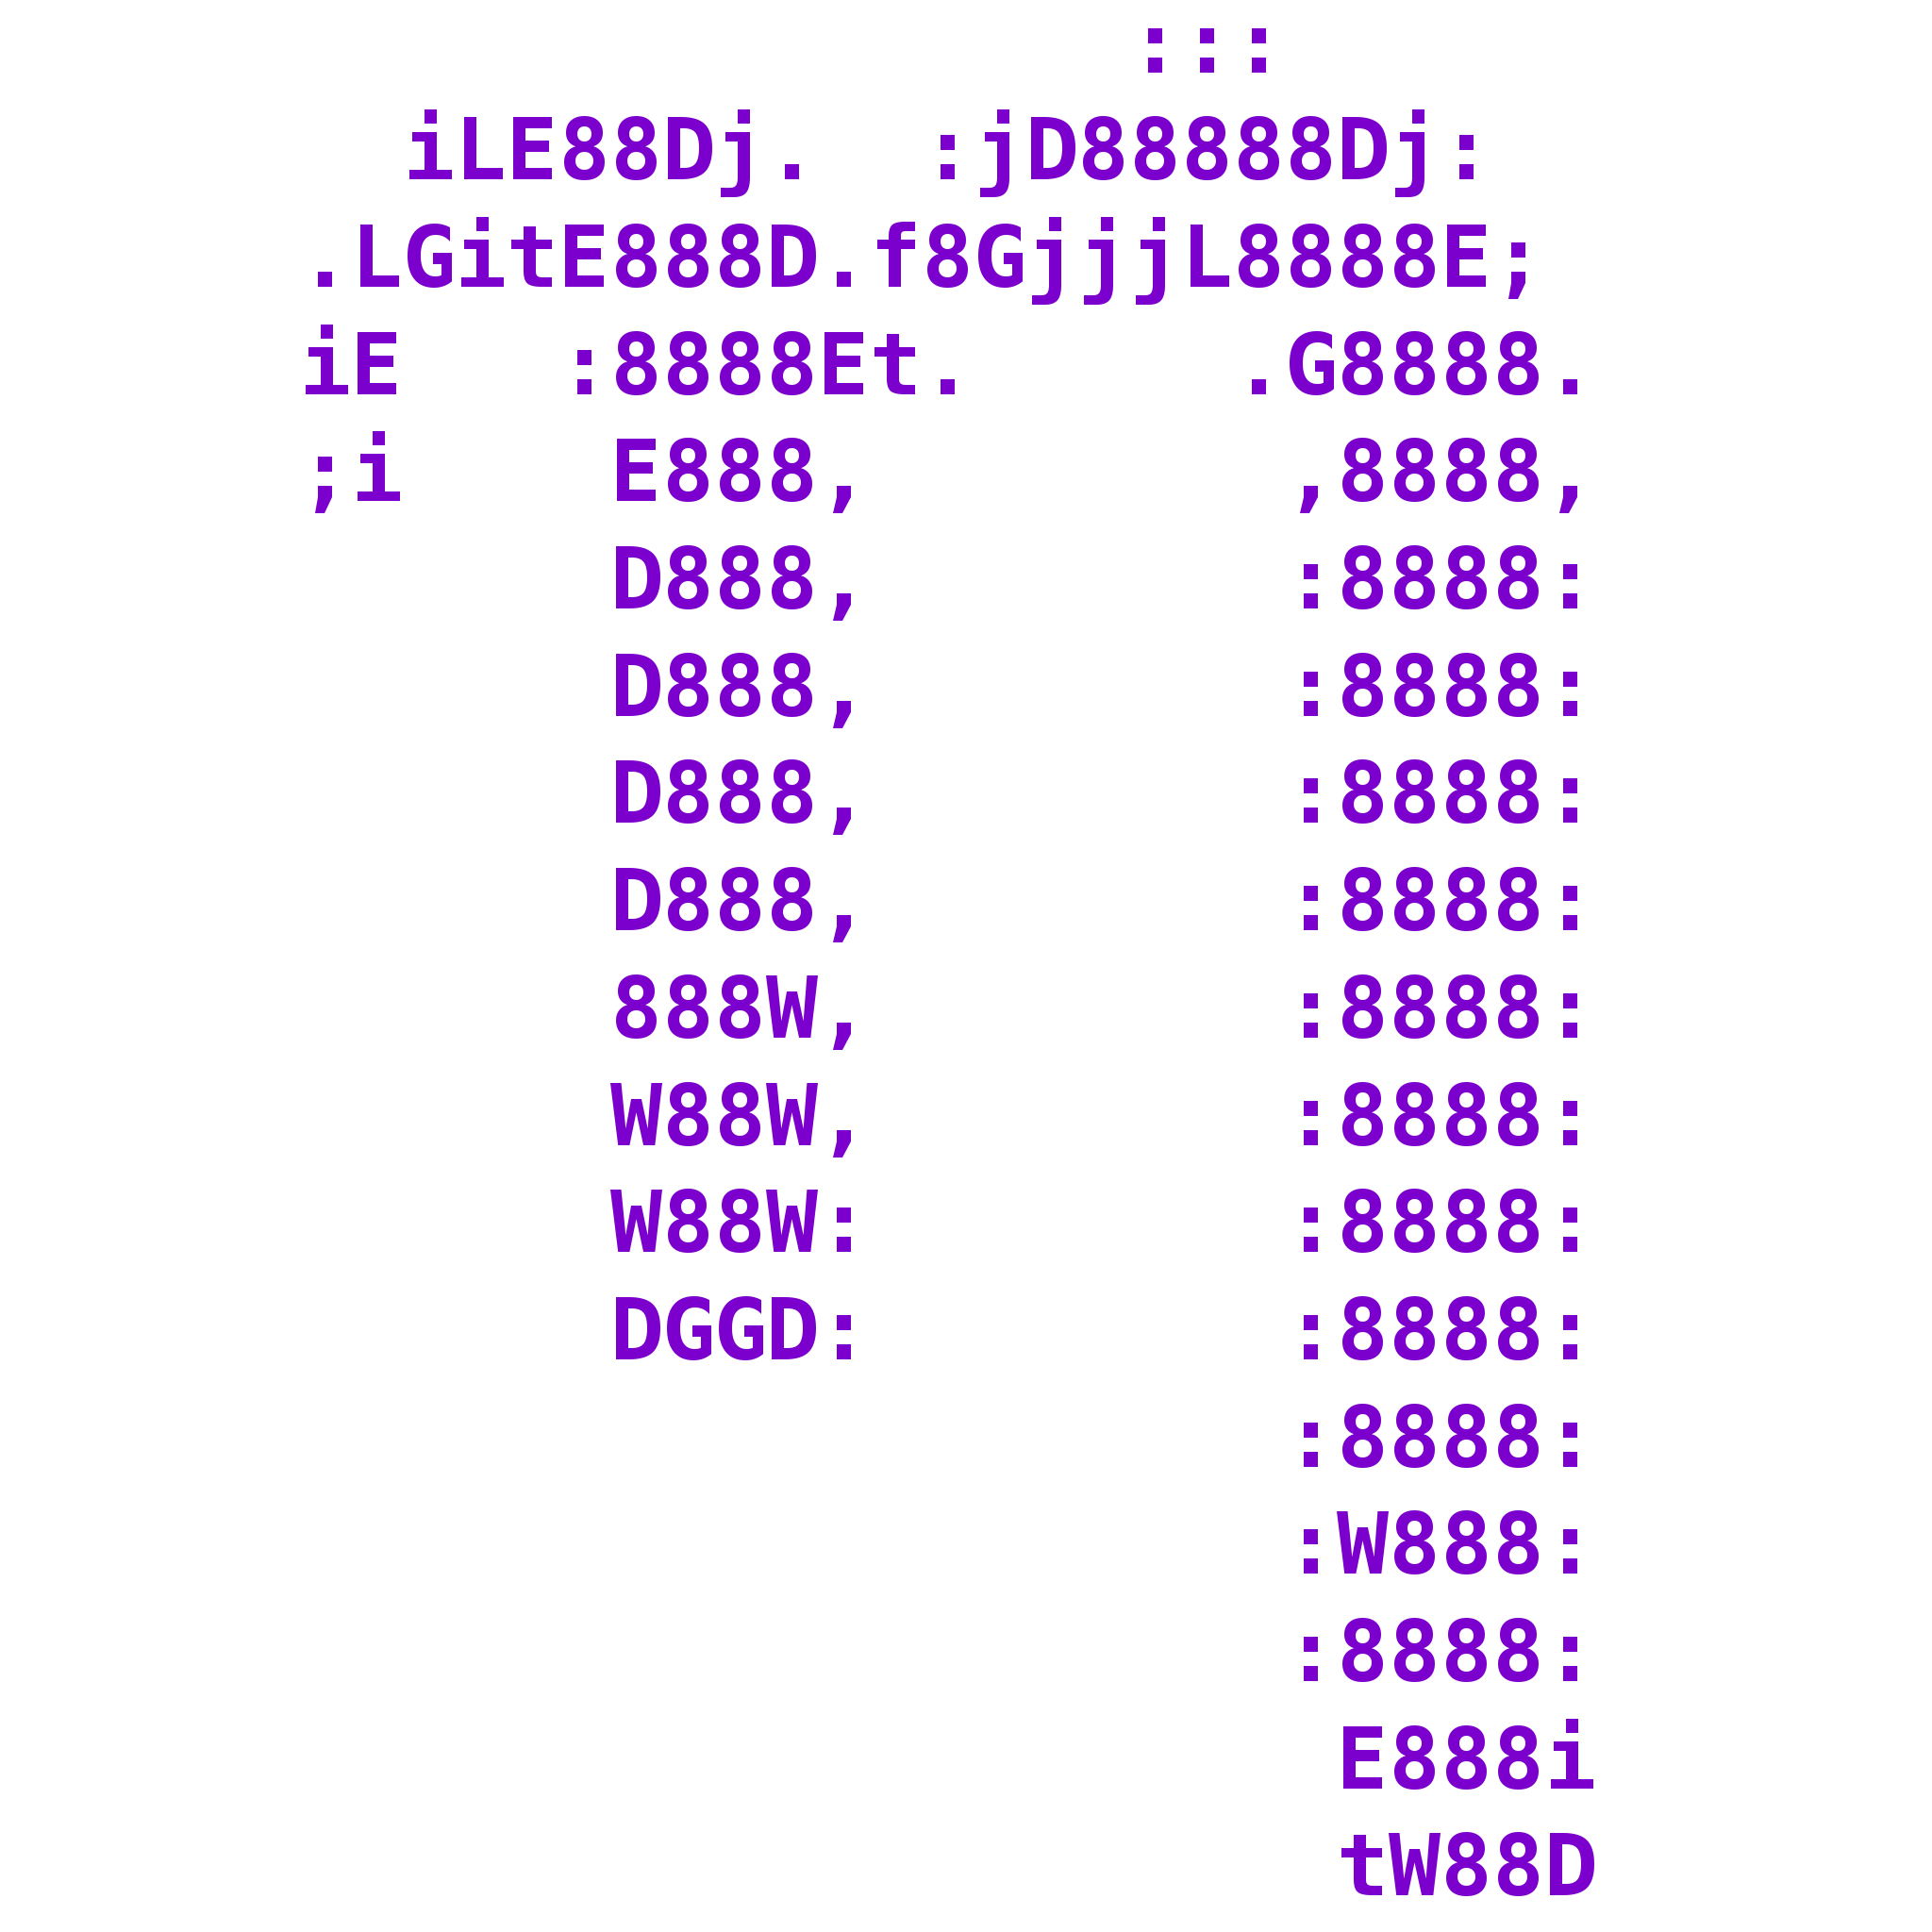
\includegraphics[width=0.2\textwidth]{img/nano_logo.png} 
			\hspace{0.5cm}
			
\includegraphics[width=0.2\textwidth]{img/Emacs_logo.png} 
	\end{figure}
\end{frame}

% Nano Text Editor 
\begin{frame}
	\frametitle{\textbf{GNU Nano Text Editor}}
		
	\begin{multicols}{2}
		\begin{figure}[h]
			\centering
			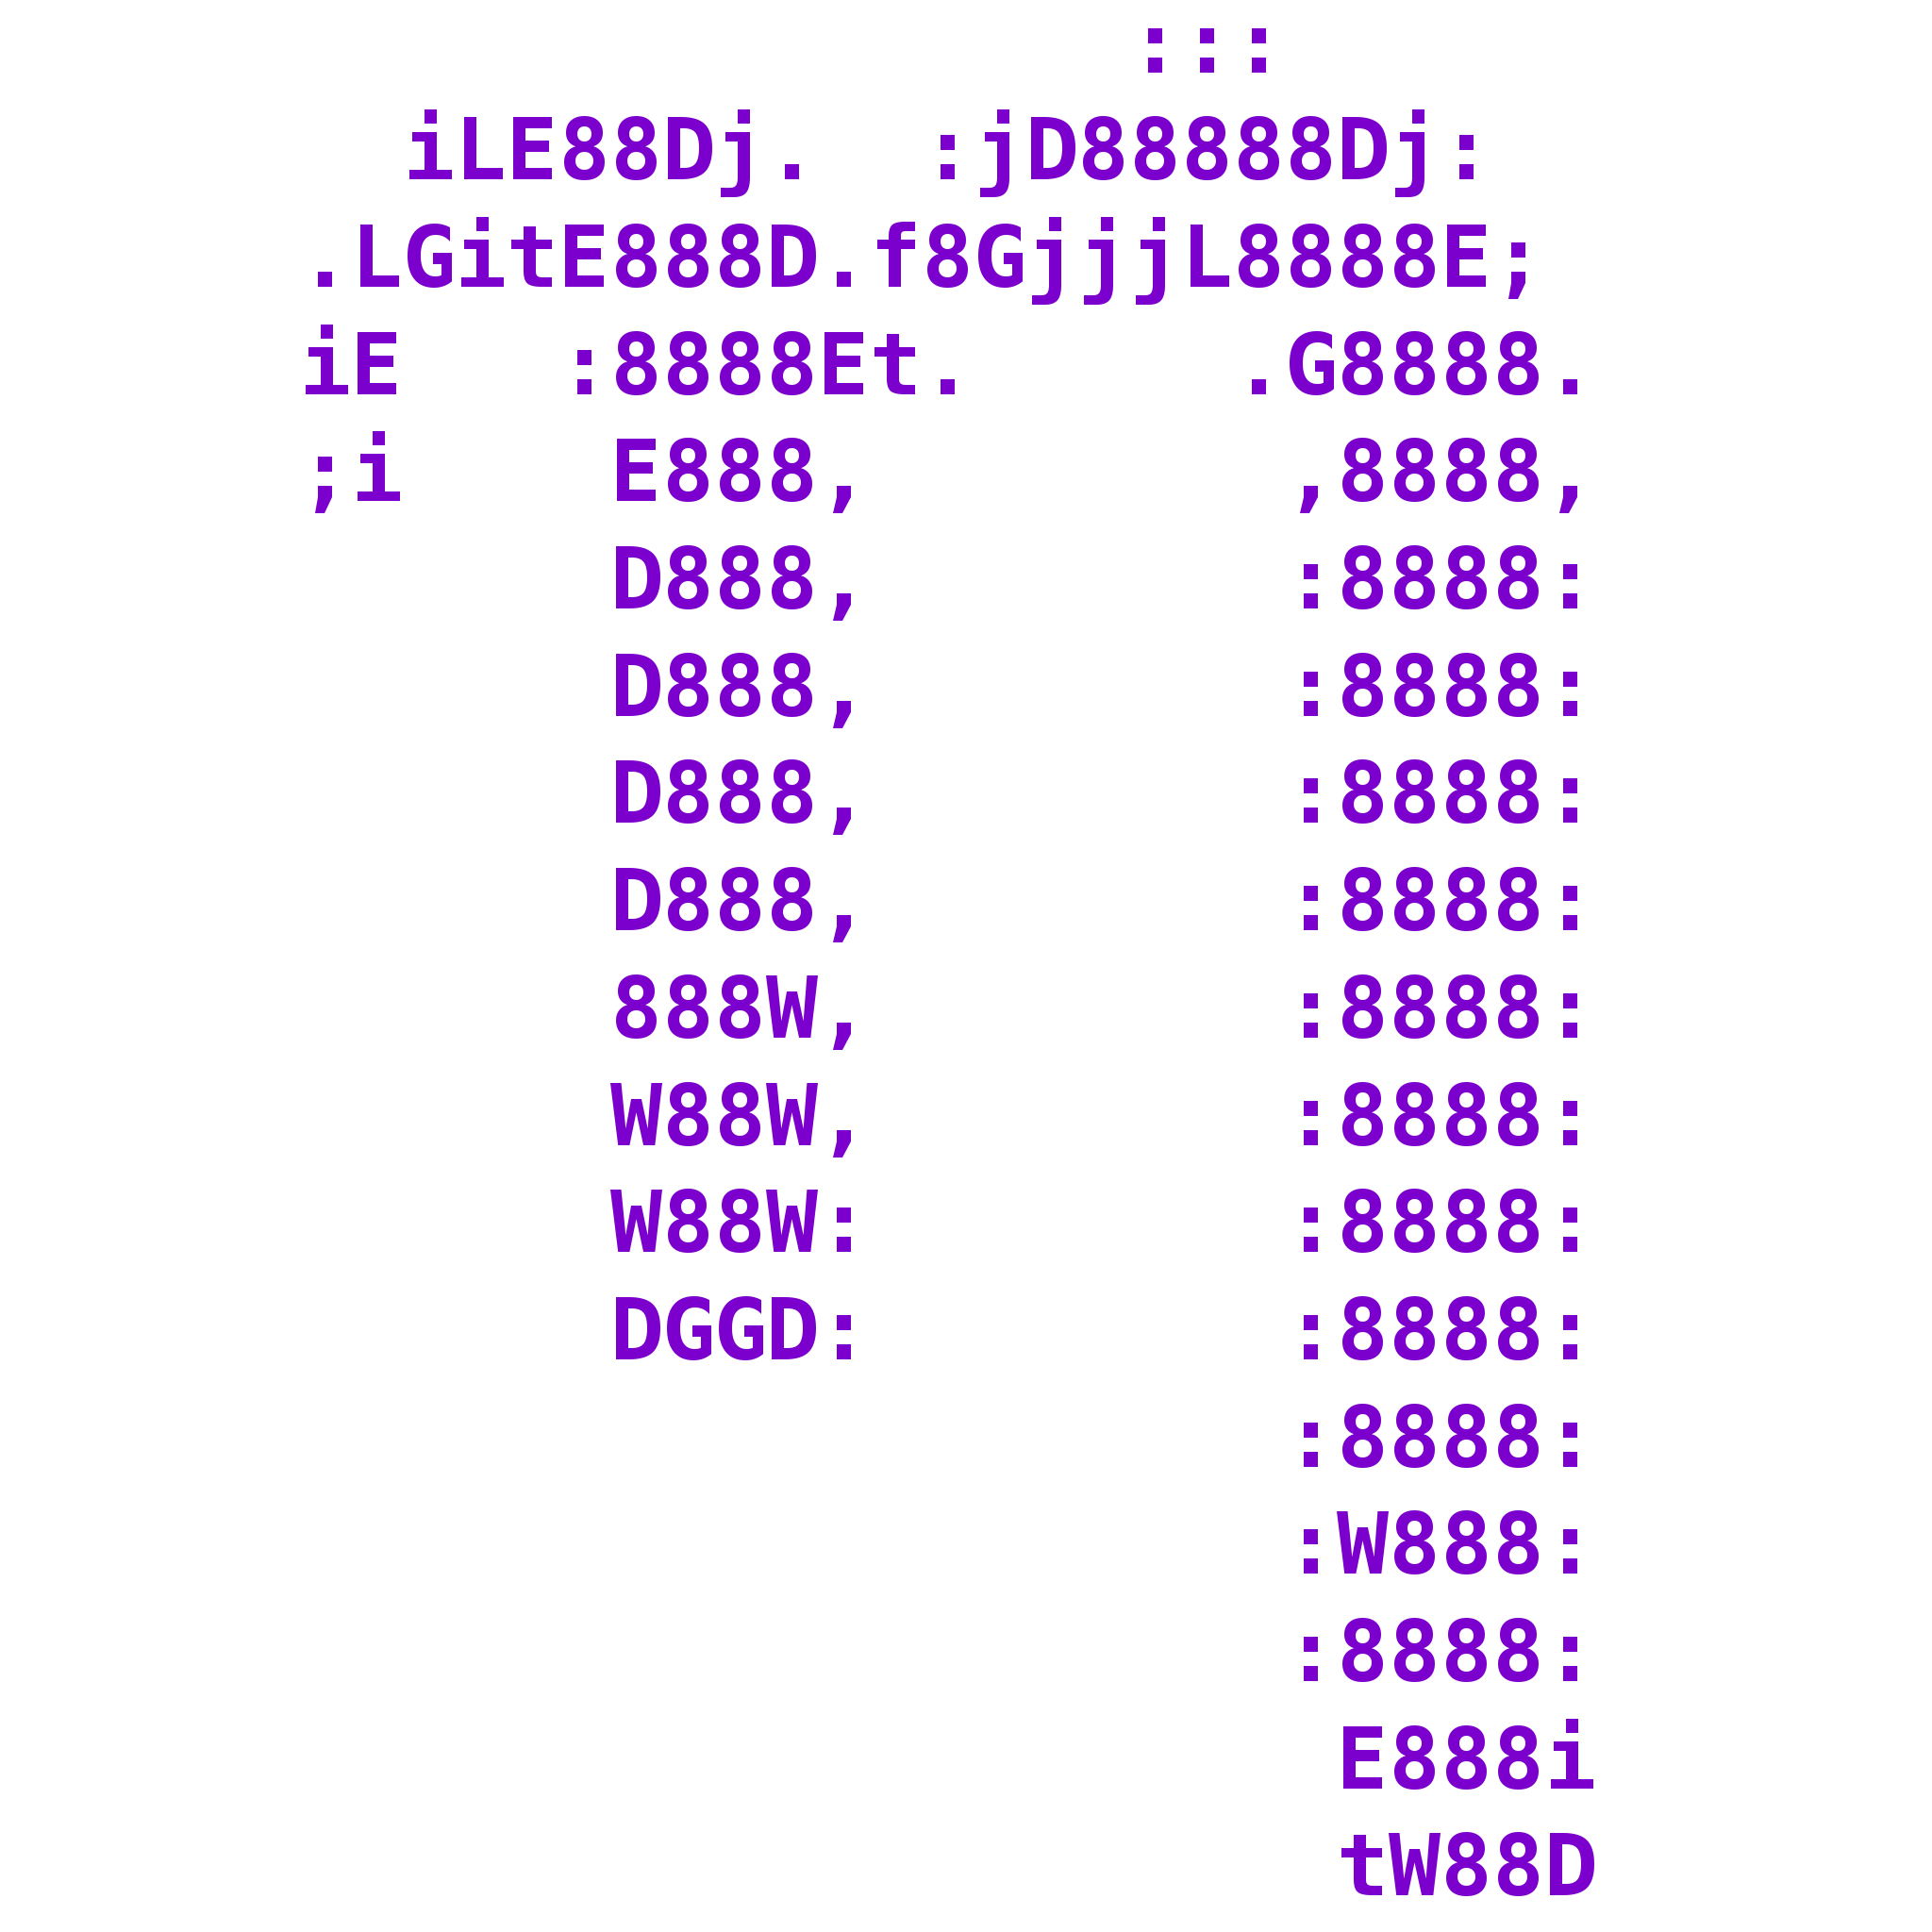
\includegraphics[width=0.2\textwidth]{img/nano_logo.png} 
		\end{figure}

		\begin{itemize}
			\item Released in November 18, 1999
			\item User-friendly and easy to learn 
			\item Developed and maintained by volunteers
		\end{itemize}

		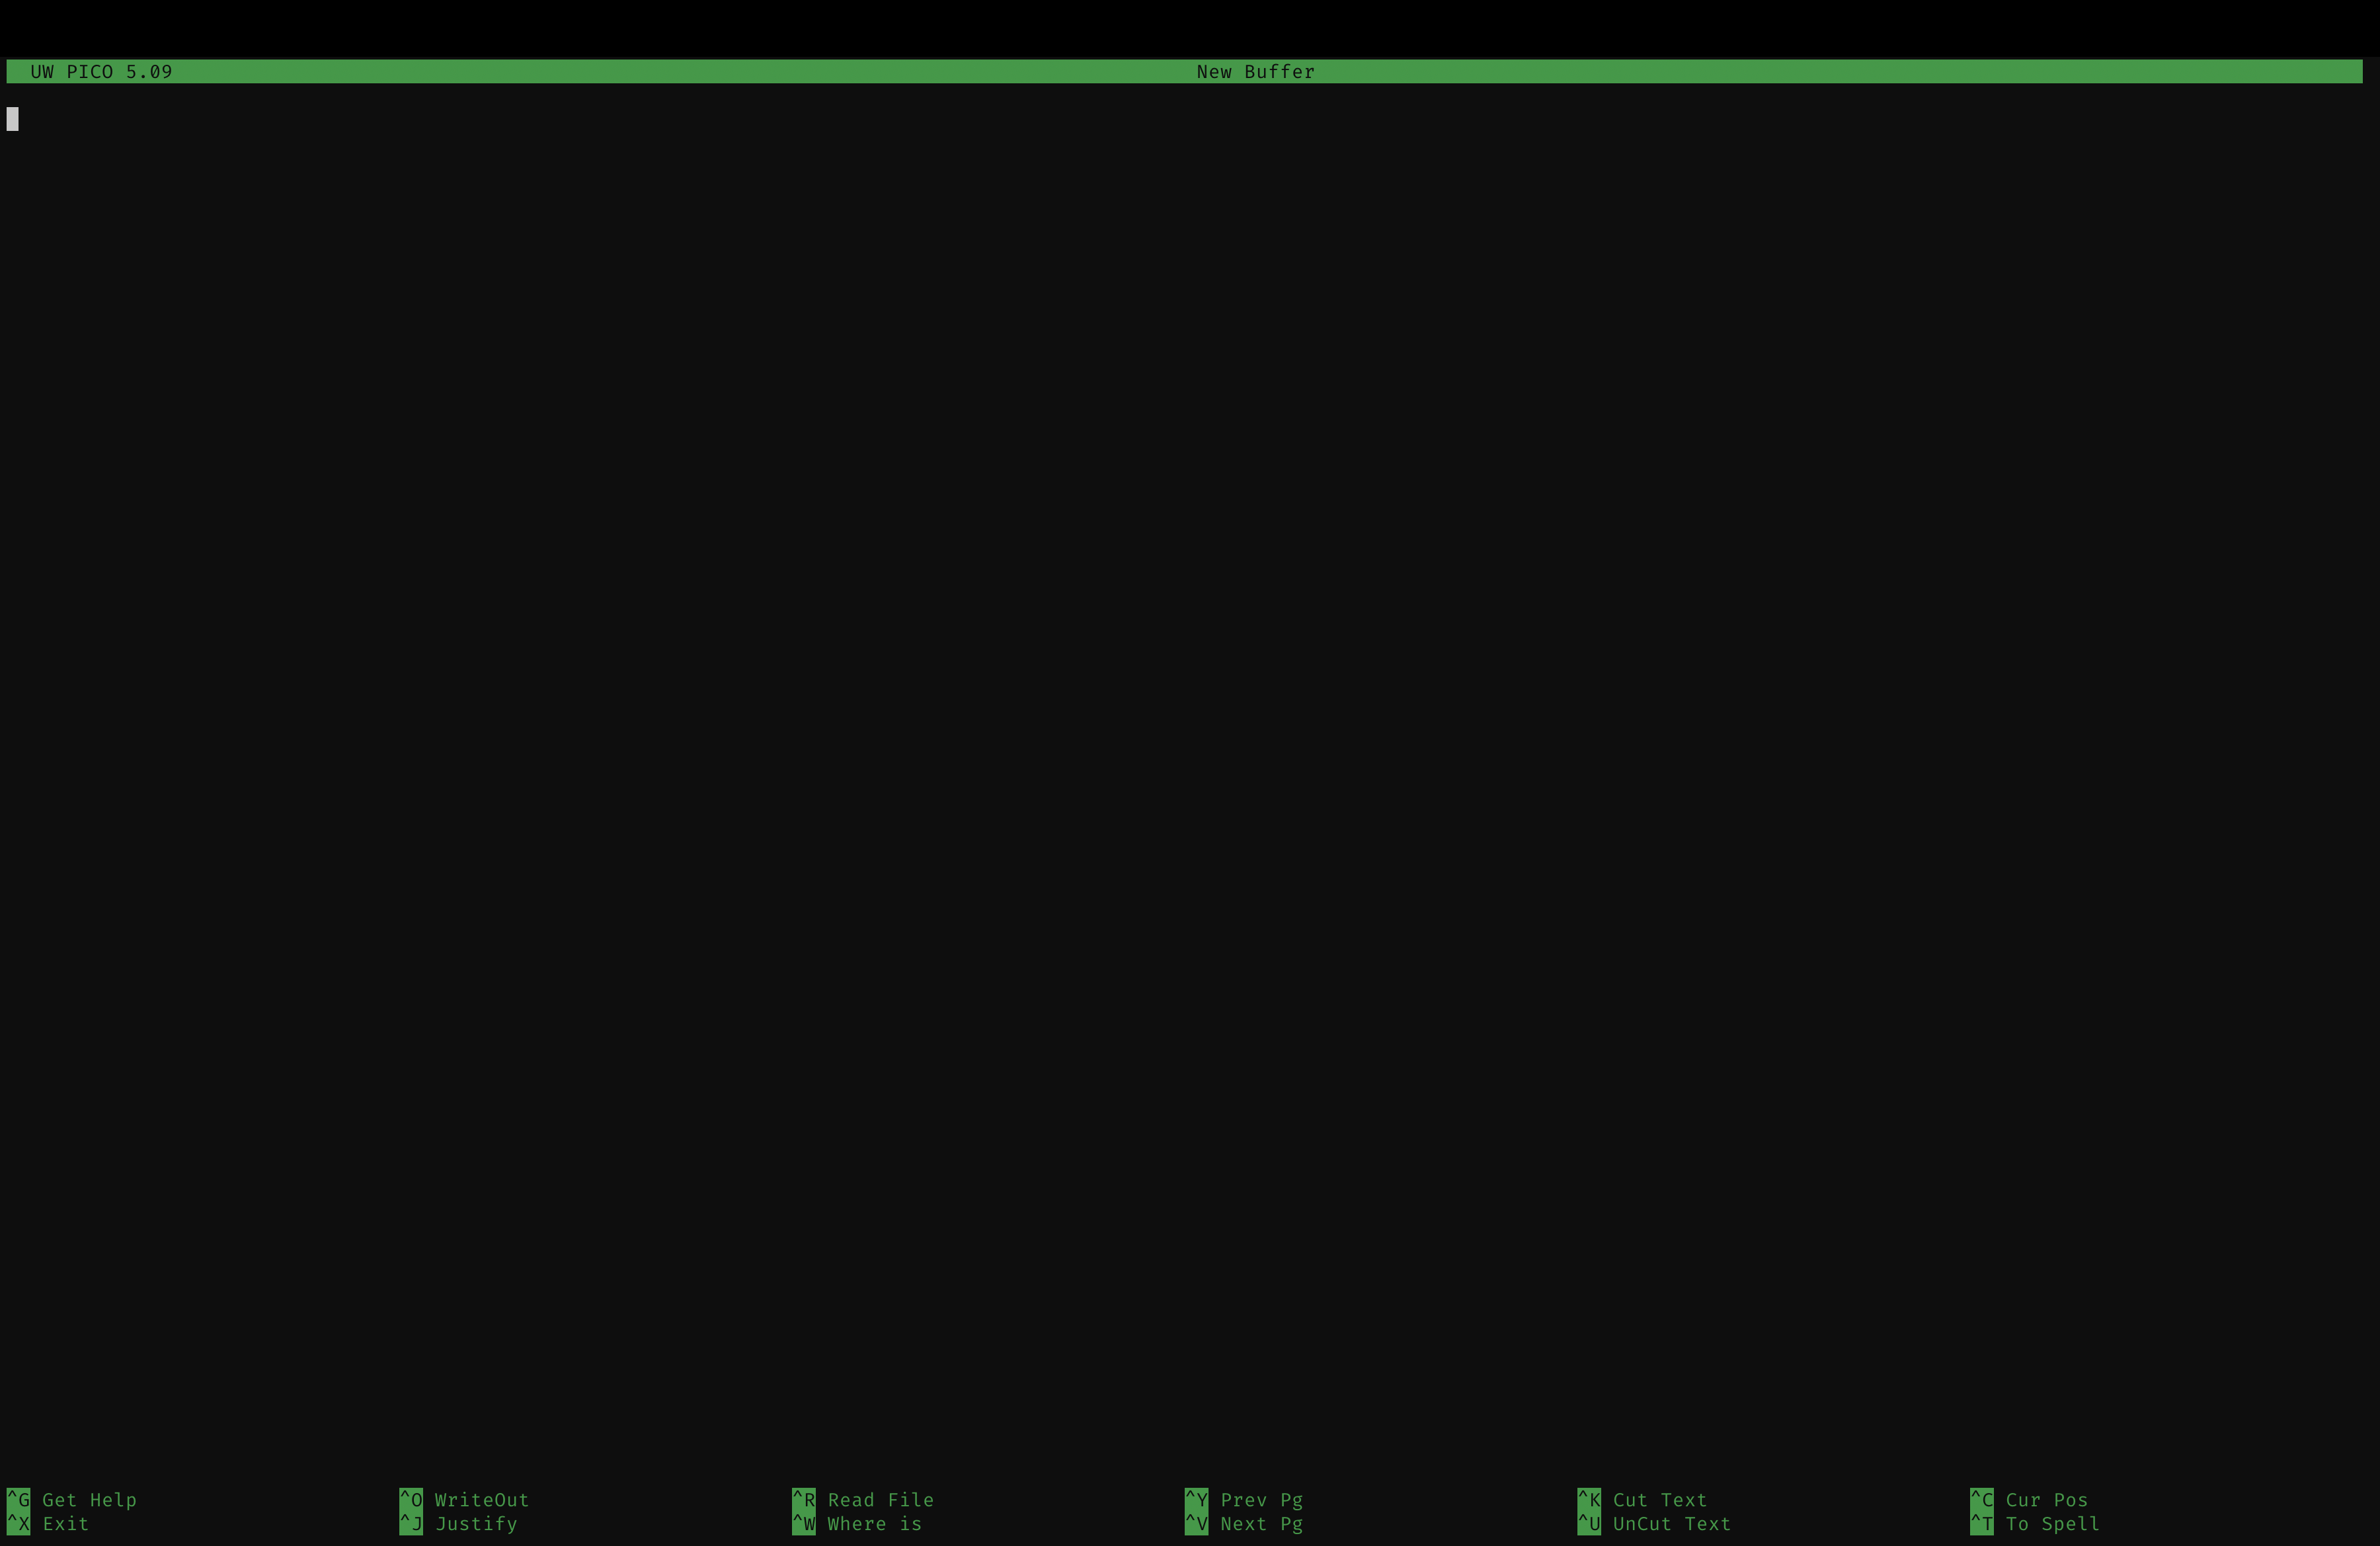
\includegraphics[width=0.5\textwidth]{img/nano.png} 
	\end{multicols}

\end{frame}

% Vim Text Editor 
\begin{frame}
	\frametitle{\textbf{Vim Text Editor}}
		
	\begin{multicols}{2}
		\begin{figure}[h]
			\centering
			
\includegraphics[width=0.2\textwidth]{img/Vim_logo.png} 
		\end{figure}

		\begin{itemize}
			\item Released in November 2, 1991
			\item Modal editor 
			\item Highly customizable, many plugins available 
		\end{itemize}

		\includegraphics[width=0.5\textwidth]{img/Vim.png} 
	\end{multicols}
\end{frame}

% Emacs Text Editor 
\begin{frame}
	\frametitle{\textbf{Emacs Text Editor}}
		
	\begin{multicols}{2}
		\begin{figure}[h]
			\centering
			
\includegraphics[width=0.2\textwidth]{img/Emacs_logo.png} 
		\end{figure}

		\begin{itemize}
			\item Released in March 20, 1985
			\item Created by GNU Project founder Richard Stallman
			\item Highly customizable
			\item Many modes for different purposes such as browsing the web
		\end{itemize}

		\includegraphics[width=0.5\textwidth]{img/Emacs.png} 
	\end{multicols}
\end{frame}

% What makes a good commit
\begin{frame}
	\frametitle{\textbf{What makes a good commit?}}
	
	\begin{itemize}
		\item Detailed messages that someone can read that informs others about the
changes you made to a document. 
	\end{itemize}

	\begin{figure}[h]	
		\centering
		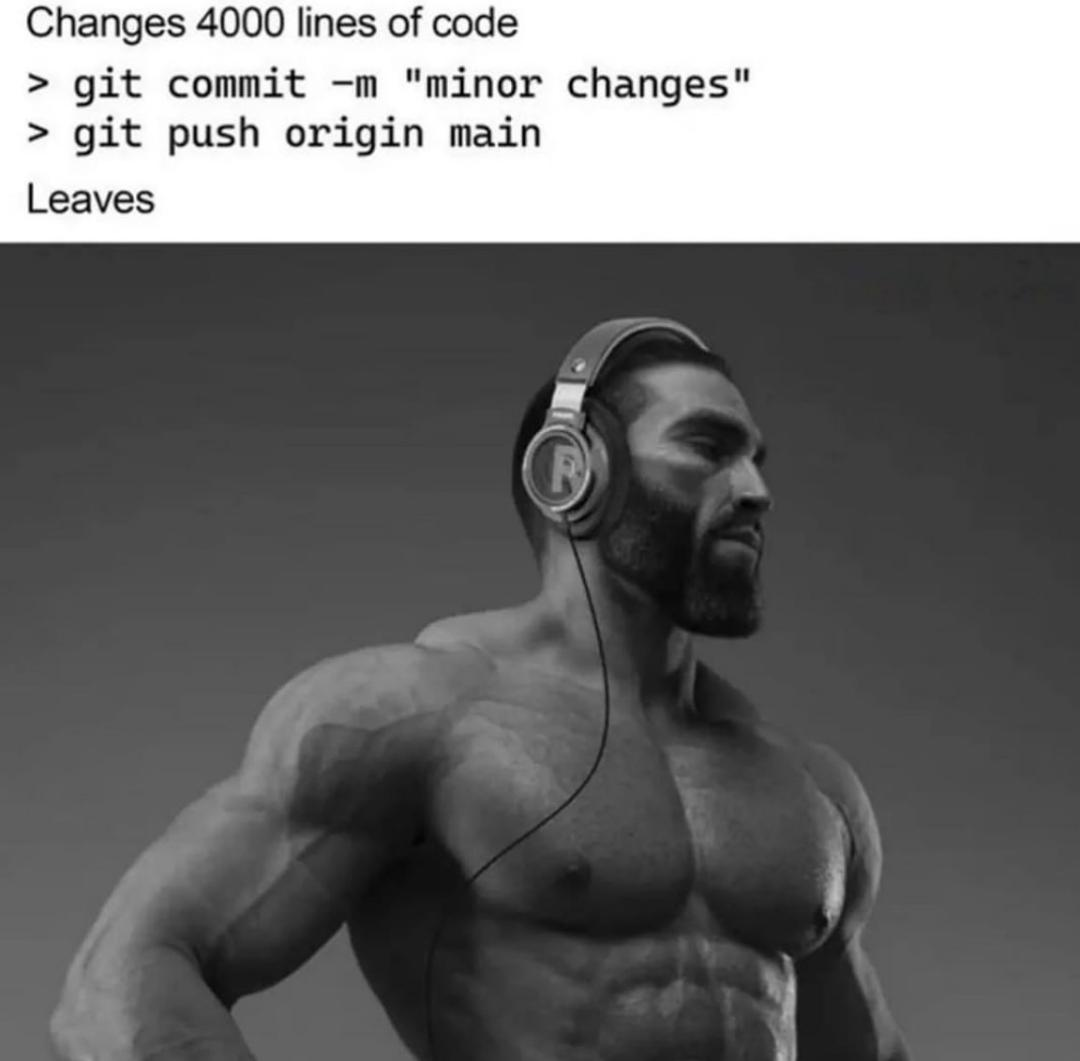
\includegraphics[width=0.5\textwidth]{img/minorchanges.jpeg} 
	\end{figure}

\end{frame}

\begin{frame} 
	\frametitle{\textbf{What makes a good commit?}}
	
	\textbf{A better approach to making commits} 
	\vspace{0.5cm}
	
	\begin{itemize}
		\item \textit{Title:} Add a topic
		\vspace{0.5cm}
		\item \textit{Changes:} Add details about changes made to file(s)
		\vspace{0.5cm}
		\item \textit{State:} Add a brief summary of the state of program or feature
		\vspace{0.5cm}
		\item \textit{TODO:} Make notes about things to fix
	\end{itemize}	

	\begin{block}{\textbf{PRO TIP}}
		Pretend you are sending an email to your friends, group mates, or professor
		informing them of the changes you made to the document.
	\end{block}

\end{frame} 

% Making a Commit 
\begin{frame}
	\frametitle{\textbf{Making a Commit}}

	\textbf{Step 1.} \textit{Add a document to staging}
	\begin{itemize}
		\item git add \(\prec document \succ\)
	\end{itemize}

	
	\vspace{0.5cm}

	\textbf{Step 2.} \textit{View documents that have been staged (Optional)}
	\begin{itemize}
		\item git status
	\end{itemize}

	
	\vspace{0.5cm}

	\textbf{Step 3.} \textit{Remove a document from staging (Optional)}
	\begin{itemize}
		\item git reset \(\prec document \succ\)
	\end{itemize}


	\vspace{0.5cm}

	\textbf{Step 4.} \textit{Record changes to repository}
	\begin{itemize}
		\item git commit
	\end{itemize}


	\vspace{0.5cm}

	\textbf{Step 5.} \textit{Upload changes to remote repository}
	\begin{itemize}
		\item git push 
	\end{itemize}
\end{frame}
\end{document}
